\documentclass[12pt]{article}
\usepackage{changepage,soul,graphicx,graphbox,stoversymb}%,afterpage}
\usepackage[left=0.5in,right=0.5in,bottom=1in,top=0.75in]{geometry}%,showframe=true
\everymath{\displaystyle}

\usepackage[many]{tcolorbox}
\usepackage[inline]{enumitem}
\usepackage{amsmath,amsthm}
	\theoremstyle{definition}
	\newtheorem{defn}{Definition}
	
	\newtheoremstyle{underl}{4.5mm}{4.5mm}{}{}{}{\textnormal{.}}{ }{\underline{\thmname{#1}}}
	\theoremstyle{underl}
	\newtheorem*{ex}{Ex}

\thispagestyle{empty}

\newcommand{\capt}[1]{\begin{adjustwidth}{0.5in}{0.5in}\centering\small\textit{#1}\end{adjustwidth}}
\newcommand{\notebox}[2]
{\begin{tcolorbox}[
		enhanced,
		colback=white,
		colframe=black,
		boxrule=0.5pt,
		arc=0pt,
		top=3mm,
		bottom=3mm, 
		grow to left by=-0.5in,
		grow to right by=-0.5in
	]
	\noindent\textbf{#1}\\
	{#2}
\end{tcolorbox}}
\newcommand{\hintbf}[1]{\textbf{Hint}: #1}
\newcommand{\eqbox}[1]{\begin{tcolorbox}
		[colback=white,colframe=gray,boxrule=0.5pt,arc=0pt,top=3mm,bottom=3mm,width=4in,center]#1\end{tcolorbox}\vspace{3mm}}

\begin{document}
		\begin{enumerate}[label=(\alph*), itemsep=0.125in, topsep=3mm, leftmargin=0.25in, rightmargin=0.25in]
			\item $y=0$, $y=5$, and $y=9$
			\item $y=0$ is \textbf{stable}; $y=5$ is \textbf{unstable}; $y=9$ is \textbf{stable}.
			\item Given that $y(0)=2$, $\lim_{x\to\infty}y(x)=0$.
			\begin{itemize}[label=$\circ$]
				\item To see this, note first that $y=2$ lives in the $y$-interval $(0,5)$.
				\item Then, because $y=0$ is asymptotically stable, every integral curve in the $y$-intervals $(-\infty,0)$ \ul{and} $(0,5)$ go to 0 as $x\to\infty$.
				\item The graph of the \textbf{actual} solution (which you were told not to find) verifies our claim:
					\begin{center}
						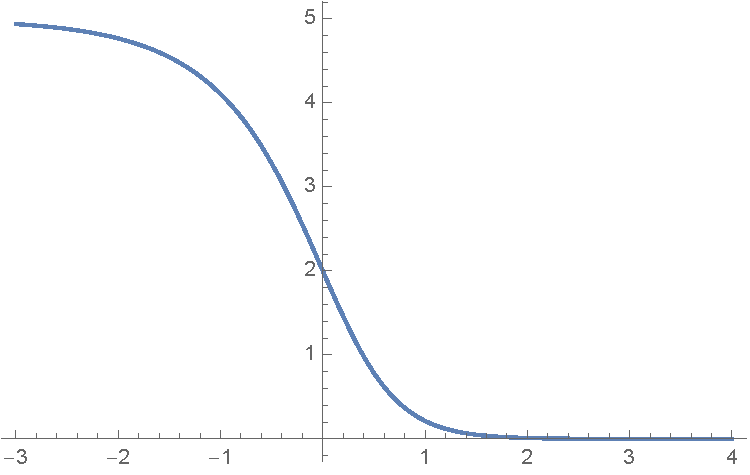
\includegraphics[scale=0.625]{curve}
					\end{center}\vspace{-6mm}
			\end{itemize} 
			\item (iv)
			\item I cheated and used the computer; \textbf{you} should do it without cheating, and upon doing so, your result should look something like this:
				\begin{center}
					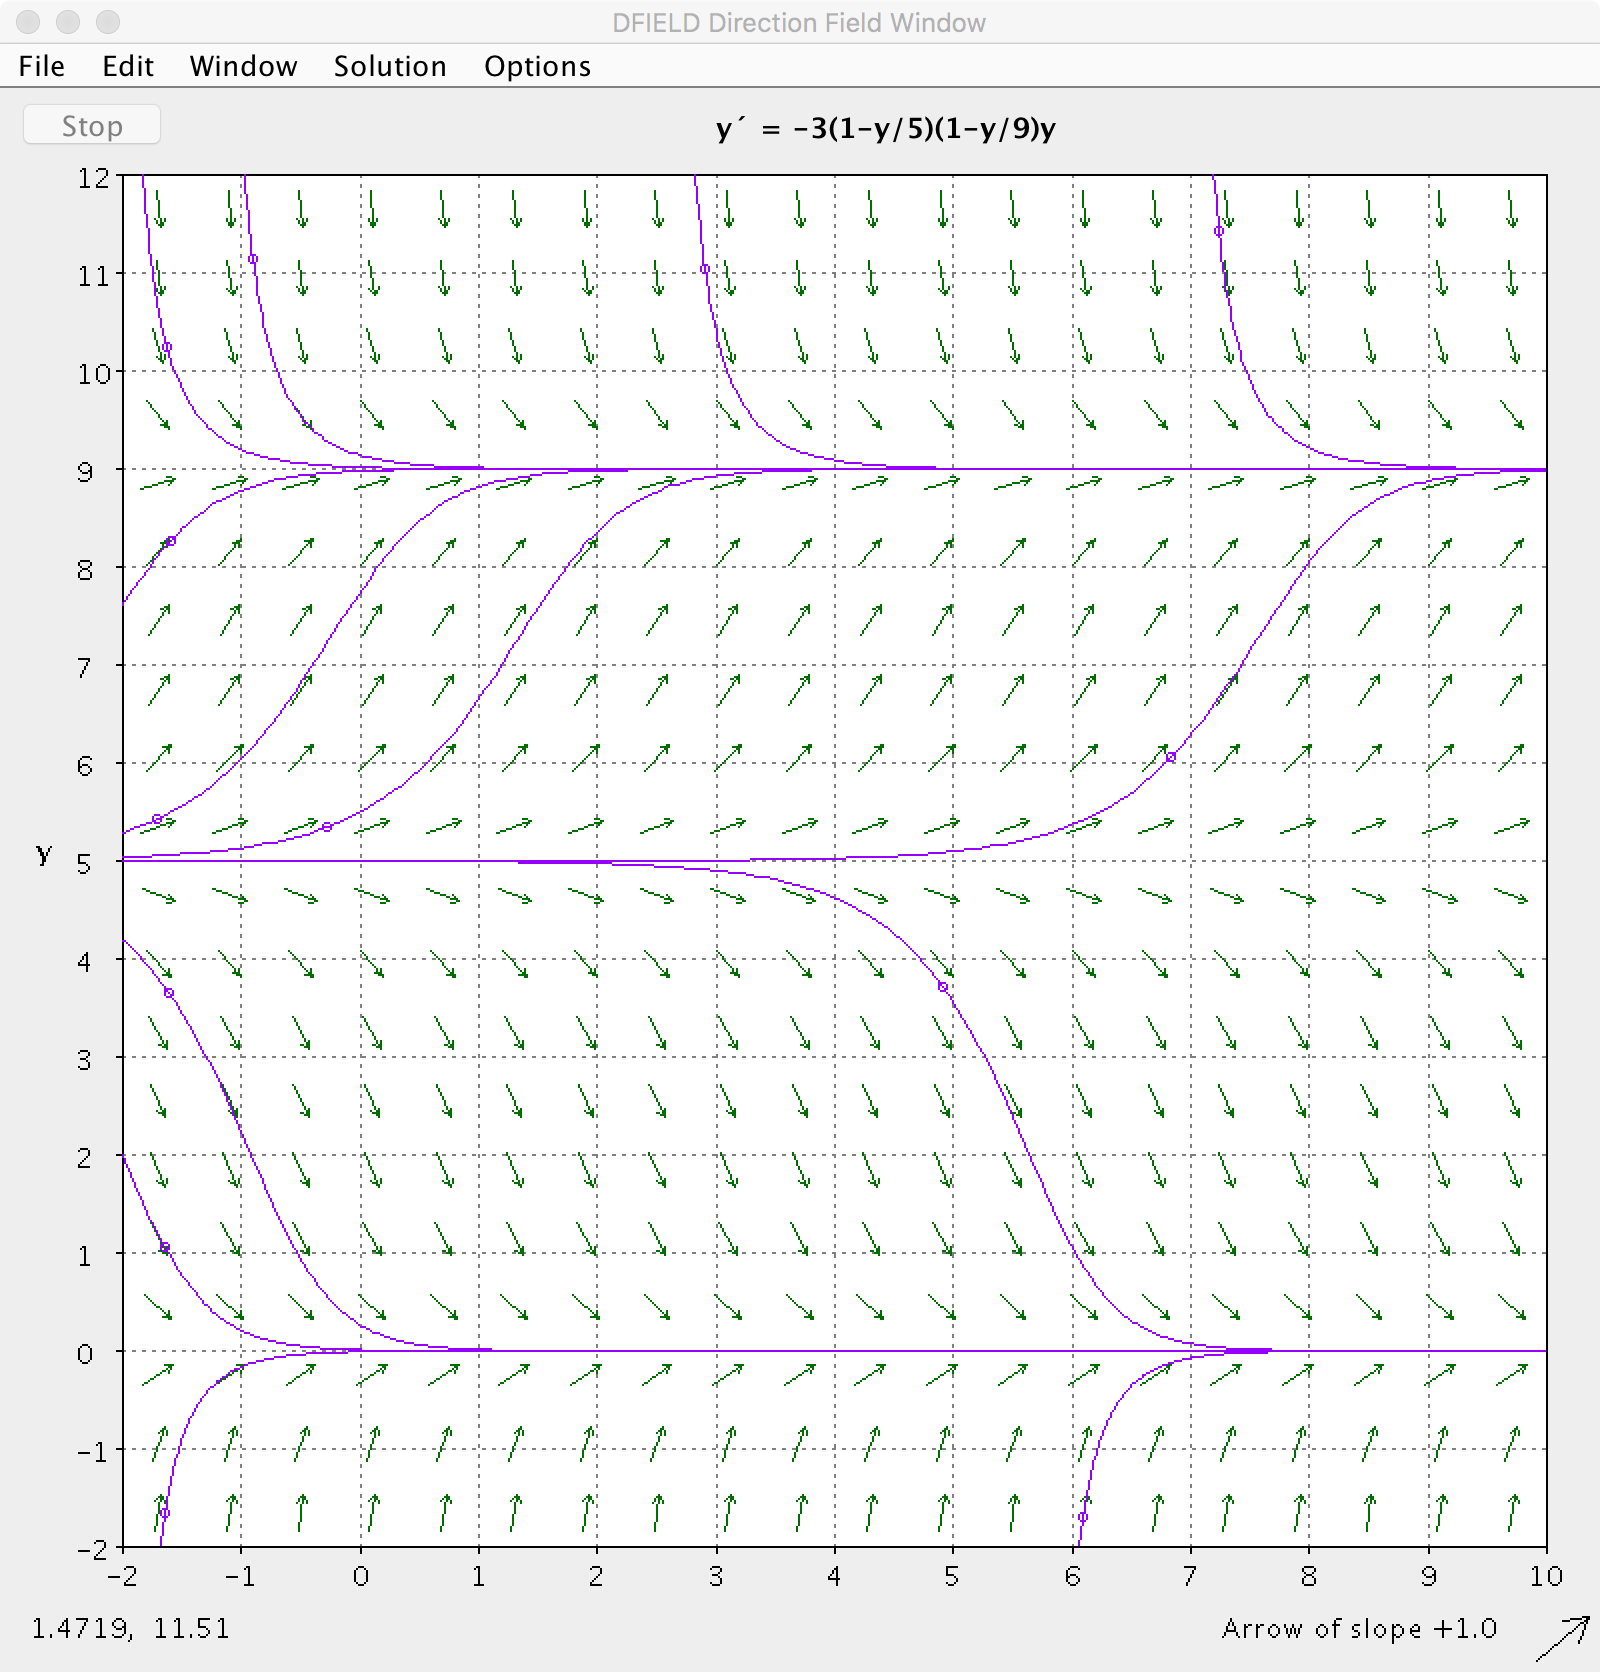
\includegraphics[scale=0.35]{HandoutDFIELD}
				\end{center}
			\item False
			\item (ii)
			\item This equation (like \textbf{every} autonomous ODE) is separable:
			$$\frac{dy}{\left(1-\frac{y}{5}\right)\left(1-\frac{y}{9}\right) y}=-3\,dx.$$
			Using partial fractions, we can decompose the lefthand side:
			$$\left(\frac{1}{y}-\frac{9}{4(y-5)}+\frac{5}{4(y-9)}\right)\,dy=-3\,dx.$$
			Now, we integrate each side:
			$$\int\left(\frac{1}{y}-\frac{9}{4(y-5)}+\frac{5}{4(y-9)}\right)\,dy=\int-3\,dx \iff \ln|y|-\frac{9}{4}\ln|y-5|+\frac{5}{4}\ln|y-9|=-3x+C.$$
			Next, we rewrite the lefthand side using properties of logarithms:
			$$\ln\left(\frac{|y|\,|y-9|^{5/4}}{|y-5|^{9/4}}\right)=-3x+C.$$
			Finally, we eliminate the $\ln$, giving a solution in implicit form:
			\eqbox{$$\frac{|y|\,|y-9|^{5/4}}{|y-5|^{9/4}}=e^{-3x+C}.$$}
			\textbf{Note:} We have to leave the absolute values here because we were told initially to allow $y<0$.
			\item After part (h) above, all that's left is to find the constant $C$ corresponding to the point $(-1,\pi)$. Doing so yields
			$$\frac{|\pi|\,|\pi-9|^{5/4}}{|\pi-5|^{9/4}}=e^{-3(-1)+C}\iff C=\ln\left(\frac{\pi(9-\pi)^{5/4}}{e^3(5-\pi)^{9/4}}\right).$$
			\vspace{1.5mm}
			
			\textbf{Note 1:} The last step used the property $e^{a+b}=e^ae^b$.\vspace{3mm}
			
			\textbf{Note 2:} We were able to remove the absolute values by rewriting accordingly. In the numerator of $C$, for example, $\pi-9<0$ implies that $|\pi-9|=-(\pi-9)$ (since absolute value makes negative things positive), and because 
			$$-(\pi-9)=9-\pi,$$
			we have that $|\pi-9|=9-\pi$ and hence that $|\pi-9|^{5/4}=(9-\pi)^{5/4}$. The same is true for the $|\pi-5|^{9/4}$ term in the denominator.
		\end{enumerate}
\end{document}